\documentclass[aspectratio=169, 10pt]{beamer}
\usepackage[fontset=fandol]{ctex}
\usepackage{amsmath, amssymb, mathtools}
\usepackage{booktabs}
\usepackage{graphicx}
\usepackage{xcolor}
\usepackage{tikz}
\usetikzlibrary{arrows.meta, positioning, shapes.geometric}

% -- Theme ---------------------------------------------------------------
\usetheme{Madrid}
\usecolortheme{dolphin}
\usefonttheme{professionalfonts}
\setbeamertemplate{navigation symbols}{}

% -- Compact spacing ------------------------------------------------------
\setbeamersize{text margin left=6mm, text margin right=6mm}
\renewcommand{\baselinestretch}{0.92}
\setlength{\parskip}{0pt}
\setbeamertemplate{itemize items}[circle]
\setbeamerfont{block title}{size=\small,series=\bfseries}
\setbeamerfont{block body}{size=\small}
\setbeamerfont{block title alerted}{size=\small,series=\bfseries}
\setbeamerfont{block body alerted}{size=\small}

% -- Colors --------------------------------------------------------------
\definecolor{myblue}{HTML}{2B5EA7}
\definecolor{accentgreen}{HTML}{2E8B57}
\definecolor{accentred}{HTML}{C0392B}
\definecolor{accentorange}{HTML}{D35400}
\definecolor{lightbg}{HTML}{F5F7FA}
\setbeamercolor{frametitle}{bg=myblue, fg=white}
\setbeamercolor{structure}{fg=myblue}
\setbeamercolor{block title}{bg=myblue!85, fg=white}
\setbeamercolor{block body}{bg=myblue!8}
\setbeamercolor{alerted text}{fg=accentred}
\setbeamercolor{block title alerted}{bg=accentred, fg=white}
\setbeamercolor{block body alerted}{bg=accentred!10}

% -- Auto section title page ---------------------------------------------
\AtBeginSection[]{
  \begin{frame}
    \vfill\centering
    \usebeamerfont{title}\textcolor{myblue}{\insertsectionhead}\par
    \vfill
  \end{frame}
}

% -- Footer with GitHub URL ----------------------------------------------
\setbeamertemplate{footline}{%
  \leavevmode%
  \hbox{%
  \begin{beamercolorbox}[wd=.55\paperwidth,ht=2.5ex,dp=1ex,leftskip=2ex]{author in head/foot}%
    \tiny\texttt{github.com/dechang64/organoid-fl}%
  \end{beamercolorbox}%
  \begin{beamercolorbox}[wd=.35\paperwidth,ht=2.5ex,dp=1ex,center]{author in head/foot}%
    \tiny\insertshorttitle%
  \end{beamercolorbox}%
  \begin{beamercolorbox}[wd=.10\paperwidth,ht=2.5ex,dp=1ex,center]{author in head/foot}%
    \tiny\insertframenumber{} / \inserttotalframenumber%
  \end{beamercolorbox}}%
  \vskip0pt%
}

% -- Metadata ------------------------------------------------------------
\title[Organoid-FL]{Organoid-FL: 类器官检测联邦学习平台}
\subtitle{项目进展汇报 v9}
\date{2026年7月}

\begin{document}

% ========================================================================
\begin{frame}[plain]
  \titlepage
\end{frame}

\begin{frame}{目录}
  \tableofcontents
\end{frame}

% ========================================================================
\section{问题与背景}

\begin{frame}{什么是类器官？}
  \begin{columns}[T]
    \column{0.55\textwidth}
    \begin{block}{类器官（Organoid）}
      \begin{itemize}
        \item 体外培养的微型器官（肺、肠、脑等）
        \item 用于药物筛选、个性化医疗、疾病建模
        \item 显微镜下成像后需\textbf{人工计数和形态分析}
        \item 通量低、主观性强、跨实验室一致性差
      \end{itemize}
    \end{block}
    \vspace{0em}
    \begin{alertblock}{核心痛点}
      类器官图像分析依赖人工，成为药物研发管线的瓶颈。
      自动化检测是解决方案，但面临多个技术挑战。
    \end{alertblock}
    \column{0.40\textwidth}
    \begin{block}{技术挑战}
      \begin{itemize}
        \item \alert{超大图}：6K$\times$5.7K 像素
        \item \alert{密集小目标}：单图数百个 organoid
        \item \alert{标注噪声}：多标注者不一致
        \item \alert{数据分散}：多中心数据无法共享
      \end{itemize}
    \end{block}
  \end{columns}
\end{frame}

\begin{frame}{为什么需要联邦学习？}
  \begin{block}{数据隐私与数据分散的矛盾}
    \begin{itemize}
      \item 多家医院/实验室各自有类器官图像数据
      \item 涉及患者来源 → \alert{无法集中共享}
      \item 单中心数据量不足 → 模型泛化性差
      \item 各中心培养条件/成像设备不同 → 数据分布异构（non-IID）
    \end{itemize}
  \end{block}
  \vspace{0em}
  \begin{block}{联邦学习（Federated Learning）}
    \begin{itemize}
      \item \textbf{数据不动，模型动}：各中心本地训练，只上传模型参数
      \item \textbf{数据不动，知识动}：聚合后的全局模型吸收所有中心的知识
      \item \textbf{数据不动，推理动}：全局模型下发给各中心本地推理
    \end{itemize}
  \end{block}
  \vspace{0em}
  \centering\alert{FL + Organoid 是未被探索的交叉方向}
\end{frame}

% ========================================================================
\section{踩坑总结}

\begin{frame}{踩坑总结：数据集层面}
  \begin{alertblock}{铁律：使用任何新数据集前，必须先查官方文档}
    \begin{itemize}
      \item MultiOrg 标注 JSON 使用 napari 的 \textbf{(row, col) = (y, x)} 坐标系，不是常规 (x, y)
      \item 论文用\textbf{单类} organoid（Normal/Macros 只是培养条件，不是检测类别）
      \item 论文用 \textbf{512 patch + 丢弃边界 bbox + 全图滑动窗口推理}，不是 640 patch 上直接评估
    \end{itemize}
  \end{alertblock}
  \vspace{0em}
  \begin{block}{三个根本性错误 → 100 epoch mAP=0}
    \begin{tabular}{p{3.5cm}p{4cm}p{4cm}}
      \toprule
      & \textbf{错误做法} & \textbf{正确做法（论文方法）} \\
      \midrule
      类别 & 2类（Normal/Macros） & \textbf{单类} organoid \\
      边界 bbox & 裁剪到 patch 边缘 & \textbf{丢弃}边界 bbox \\
      评估 & patch 上直接评估 & 全图滑动窗口推理 \\
      \bottomrule
    \end{tabular}
  \end{block}
  \vspace{0em}
  \begin{block}{坐标系错误 → 标注越界}
    napari [y,x] 格式被当 [x,y] 读 → 标注 y 最大 5845 $>$ 图片高 5720，交换后 x 最大 5845 $<$ 宽 6385 ✓
  \end{block}
\end{frame}

\begin{frame}{踩坑总结：代码层面}
  \begin{block}{2026-06-28 系统审计发现 7 个 bug}
    \begin{tabular}{p{3.2cm}p{2.5cm}p{4.5cm}p{1.2cm}}
      \toprule
      \textbf{文件} & \textbf{Bug} & \textbf{影响} & \textbf{严重性} \\
      \midrule
      multiorg\_sam2.py & mask\_iou\_cropped offset x/y 交换 & 所有 mask mAP 数值错误 & \alert{Critical} \\
      multiorg\_sam2.py & mask\_iou() 死代码 & 无 & Minor \\
      multiorg\_sam2.py & load\_sam2 临时文件不清理 & 磁盘泄漏 & Medium \\
      multiorg\_tiling\_v3.py & PIL I;16→numpy segfault & Macros 类崩溃 & \alert{Critical} \\
      prepare\_sam2\_pseudo.py & cache return 跳过所有后续图 & 数据缺失 & \alert{Critical} \\
      prepare\_sam2\_pseudo.py & fallback mask 全图分配 & OOM 风险 & Medium \\
      prepare\_sam2\_pseudo.py & instance 编号错位 & 训练读错 mask & \alert{Critical} \\
      \bottomrule
    \end{tabular}
  \end{block}
  \vspace{0em}
  \begin{alertblock}{教训}
    \begin{itemize}
      \item 写完脚本必须端到端验证，不能只过 py\_compile
      \item offset/坐标格式必须统一标注 (x,y) 还是 (y,x)
      \item docstring 里的路径不能编造，必须从训练日志确认
    \end{itemize}
  \end{alertblock}
\end{frame}

\begin{frame}{踩坑总结：实验设计层面}
  \begin{block}{val 集 drop\_boundary 导致 mAP 暴跌 15pp}
    \begin{itemize}
      \item train 用 drop\_boundary=True（干净信号）✓
      \item val 也用 drop\_boundary=True → \alert{把模型正确检测变 false positive}
      \item 正确做法：val 必须 clip 到 patch 边缘（保留所有 GT）
    \end{itemize}
  \end{block}
  \vspace{0em}
  \begin{block}{GT 标注质量决定微调策略}
    \begin{tabular}{p{2.5cm}p{4cm}p{4cm}}
      \toprule
      & \textbf{鼠肝} & \textbf{MultiOrg} \\
      \midrule
      标注类型 & 红色折线（精确轮廓） & 4点多边形（位置标注） \\
      SAM2 微调 & \textbf{有效}（F1=93.9\%） & \textbf{有害}（mask mAP -4pp） \\
      正确做法 & mask supervision & 位置 prompt only \\
      \bottomrule
    \end{tabular}
  \end{block}
  \vspace{0em}
  \begin{alertblock}{核心教训}
    用粗糙 GT 微调精确 SAM2 = 负优化。GT 质量决定 supervision 方式。
  \end{alertblock}
\end{frame}

% ========================================================================
\section{Intestinal Organoid 实验（最早）}

\begin{frame}{Intestinal Organoid：最早的类器官实验（2026-06）}
  \begin{block}{Deliod 数据集}
    \begin{itemize}
      \item 肠道类器官（intestinal organoid）检测数据集
      \item Deliod 论文 SOTA: YOLOv8s/1088/300ep $\to$ mAP50=85.7\%
      \item 关键发现: imgsz=1088（非640）是高分辨率检测的关键
    \end{itemize}
  \end{block}
  \vspace{0em}
  \begin{block}{我们的实验结果}
    \begin{tabular}{lcccc}
      \toprule
      \textbf{配置} & \textbf{mAP50} & \textbf{mAP50-95} & \textbf{vs Deliod} & \textbf{备注} \\
      \midrule
      yolo12n/1088 & 86.7\% & — & +1.0pp & 代差红利 \\
      \textbf{yolo12s+freebies} & \textbf{88.1\%} & \textbf{62.1\%} & \textbf{+2.4pp} & best=ep57 \\
      yolo12s+freebies v2 & 88.4\% & 62.2\% & +2.7pp & close\_mosaic 时序问题 \\
      yolo12m/896 & — & — & — & 20.2M 参数, 训练中 \\
      \bottomrule
    \end{tabular}
  \end{block}
  \vspace{0em}
  \begin{columns}[T]
    \column{0.48\textwidth}
    \begin{alertblock}{超 SOTA：YOLOv12 + freebies}
      copy\_paste=1.0, mixup=0.15, label\_smoothing=0.1, cos\_lr, close\_mosaic=15 \\
      \textbf{88.1\% $>$ Deliod 87.5\%}（+0.6pp）
    \end{alertblock}
    \column{0.48\textwidth}
    \begin{block}{失败实验}
      SAHI: $-$11pp; TTA: +0pp; 下采样: $-$8pp
    \end{block}
  \end{columns}
\end{frame}

% ========================================================================
\section{MultiOrg 实验结果}

\begin{frame}{标注者选择对评估的影响}
  \begin{block}{同一模型，不同标注者评估}
    \begin{tabular}{lcccc}
      \toprule
      标注者 & Instances & mAP@0.5 & mAP@0.5:0.95 & Recall \\
      \midrule
      t0（初始） & 6465 & 66.9\% & 32.6\% & 60.2\% \\
      t1\_A（二次） & 3950 & 70.5\% & 38.7\% & 64.8\% \\
      \textbf{t1\_B（最精准）} & 4112 & \textbf{78.9\%} & \textbf{53.9\%} & \textbf{72.3\%} \\
      \bottomrule
    \end{tabular}
  \end{block}
  \vspace{0em}
  \begin{alertblock}{关键发现}
    \begin{itemize}
      \item 标注者选择可造成 \textbf{12pp mAP@0.5 差异}（66.9\% vs 78.9\%）
      \item t0 噪声最大（6465 instances，含误标）；t1\_B 最精简（4112 instances）
      \item \textbf{评估方法论和模型本身一样重要}——噪声标注会严重低估模型能力
    \end{itemize}
  \end{alertblock}
\end{frame}

\begin{frame}{MultiOrg 检测精度 vs SOTA}
  \begin{block}{mAP@0.5 对比（t1\_b 标注）}
    \begin{tabular}{lcc}
      \toprule
      配置 & mAP@0.5 & vs SOTA \\
      \midrule
      Faster R-CNN（论文） & 68.4\% & $-$5.5pp \\
      YOLOv3（论文） & 70.3\% & $-$3.6pp \\
      RTMDet（论文） & 63.2\% & $-$10.7pp \\
      \textbf{SSD（论文 SOTA）} & \textbf{73.9\%} & — \\
      \midrule
      YOLOv12s patch 级 & 78.1\% & +4.2pp \\
      RF-DETR SAHI+Soft-NMS & 77.15\% & +3.3pp \\
      \textbf{RF-DETR ensemble baseline} & \textbf{77.8\%} & \textbf{+3.9pp} \\
      \bottomrule
    \end{tabular}
  \end{block}
  \vspace{0em}
  \begin{alertblock}{结论}
    \begin{itemize}
      \item \textbf{我们已是 MultiOrg SOTA}，超论文最优 SSD +3.9pp
      \item 论文 2024.10 发表，无后续工作超过我们
      \item 距 80\% 门槛差 2.2pp，瓶颈是数据量（356张 vs Orga-Dete 4008张）
    \end{itemize}
  \end{alertblock}
\end{frame}

\begin{frame}{SAM2 分割实验：自蒸馏方案}
  \begin{block}{问题：4点多边形 GT 太粗糙}
    MultiOrg 标注只标 4 个点（位置），不是精确轮廓。直接用 4点多边形微调 SAM2 = 负优化（mask mAP -4pp）。
  \end{block}
  \vspace{0em}
  \begin{block}{方案 A：自蒸馏（Self-Distillation）}
    \begin{enumerate}
      \item GT 4点多边形 → bbox（位置 prompt）
      \item SAM2 zero-shot 用 bbox 做 prompt → 伪 mask（精确轮廓）
      \item 伪 mask 作为微调 supervision（替代粗糙的 4点多边形）
    \end{enumerate}
  \end{block}
  \vspace{0em}
  \begin{block}{训练结果（5 epoch, 3060 12GB）}
    \begin{tabular}{ccccc}
      \toprule
      Epoch & Train IoU & Val IoU & Val Dice & 耗时 \\
      \midrule
      1 & 0.8437 & 0.8419 & 0.9074 & 70min \\
      3 & 0.8646 & 0.8594 & 0.9181 & 70min \\
      \textbf{5} & \textbf{0.8814} & \textbf{0.8720} & \textbf{0.9255} & 70min \\
      \bottomrule
    \end{tabular}
  \end{block}
\end{frame}

\begin{frame}{SAM2 对照实验结果}
  \begin{block}{全量 55 张测试，mask IoU bug 修复后}
    \begin{tabular}{lcccc}
      \toprule
      \textbf{配置} & \textbf{bbox mAP50} & \textbf{mask mAP50} & \textbf{F1} & \textbf{FP} \\
      \midrule
      Zero-shot SAM2 & 77.15\% & \textbf{76.39\%} & 43.9\% & 11553 \\
      Finetuned v2 (4点GT) & 77.15\% & 75.98\% & 43.9\% & 11553 \\
      Finetuned pseudo & 77.13\% & 75.89\% & 43.9\% & 11553 \\
      \bottomrule
    \end{tabular}
  \end{block}
  \vspace{0em}
  \begin{alertblock}{结论：微调 = 负优化}
    \begin{itemize}
      \item bbox mAP50 三者一致（SAM2 不改检测框）
      \item mask mAP50：zero-shot 76.39\% $>$ finetuned 75.98\% $>$ pseudo 75.89\%
      \item 根因：4 点粗糙 GT 微调精确 SAM2 = 负优化
      \item 自蒸馏天花板 = zero-shot 本身质量
    \end{itemize}
  \end{alertblock}
  \vspace{0em}
  \begin{block}{FP 抑制全面失败}
    \begin{tabular}{lc}
      \toprule
      方案 & 结论 \\
      \midrule
      形态学过滤 (circ/solid/ar) & 砍 FP $<$ 2\%，无效 \\
      DINOv2+DPMM 二级验证 & PR-AUC=0.29 $<$ 随机 0.5，完全不可分 \\
      HNM (Hard Negative Mining) & 灾难性遗忘，mAP 暴跌 40pp \\
      \bottomrule
    \end{tabular}
  \end{block}
\end{frame}

% ========================================================================
\section{鼠肝实验结果}

\begin{frame}{鼠肝实验：三批数据}
  \begin{block}{数据概况}
    \begin{tabular}{lcccc}
      \toprule
      \textbf{批次} & \textbf{张数} & \textbf{分辨率} & \textbf{Organoids} & \textbf{日期} \\
      \midrule
      Batch 1 & 10 & 2592$\times$1944 & 23 & 2026-01 \\
      Batch 2 & 10 & 2592$\times$1944 & 23 & 2026-05 \\
      Batch 3 & 20 & 4000$\times$3000 & 40 & 2026-07 \\
      \midrule
      \textbf{Total} & \textbf{40} & \textbf{2种分辨率} & \textbf{86} & \\
      \bottomrule
    \end{tabular}
  \end{block}
  \vspace{0em}
  \begin{columns}[T]
    \column{0.48\textwidth}
    \begin{block}{标注方式}
      \begin{itemize}
        \item 红色折线轮廓（精确轮廓）
        \item OpenCV 提取 → YOLO 格式 bbox
        \item 三批数据统一格式
      \end{itemize}
    \end{block}
    \column{0.48\textwidth}
    \begin{alertblock}{SOTA Benchmark}
      \begin{itemize}
        \item RF-DETR few-shot + SAM2
        \item Batch 1: F1=\textbf{93.9\%}
        \item 冬生本地 GPU
      \end{itemize}
    \end{alertblock}
  \end{columns}
\end{frame}

\begin{frame}{鼠肝 Batch 1：最早实验结果（2026-06）}
  \begin{block}{实验设计：RF-DETR few-shot + SAM2 zero-shot}
    \begin{itemize}
      \item Batch 1（10张, 2592$\times$1944, 2026-01）$\to$ 6 train + 2 test
      \item RF-DETR Small (COCO) + SAM2 zero-shot (bbox prompt)
    \end{itemize}
  \end{block}
  \vspace{0em}
  \begin{columns}[T]
    \column{0.48\textwidth}
    \begin{block}{检测结果（RF-DETR bbox）}
      \begin{tabular}{lc}
        \toprule
        \textbf{指标} & \textbf{Batch 1 test} \\
        \midrule
        TP & 7 \\
        FP & 0 \\
        FN & 0 \\
        Precision & \textbf{1.00} \\
        Recall & \textbf{1.00} \\
        F1 & \textbf{1.00} \\
        \bottomrule
      \end{tabular}
    \end{block}
    \column{0.48\textwidth}
    \begin{block}{分割结果（SAM2 mask）}
      \begin{tabular}{lc}
        \toprule
        \textbf{指标} & \textbf{Batch 1 test} \\
        \midrule
        mask F1 & \textbf{93.9\%} \\
        mask IoU (TP) & 0.872 \\
        \bottomrule
      \end{tabular}
    \end{block}
  \end{columns}
  \vspace{0em}
  \begin{alertblock}{意义}
    RF-DETR + SAM2 管线可行。红色折线标注 $\to$ SAM2 zero-shot 即可高精度。
  \end{alertblock}
\end{frame}

\begin{frame}{鼠肝实验：三方案结果 (YOLOv12n, CPU)}
  \begin{alertblock}{方案1: 跨域推理 (Batch1 训练 → Batch2/3 推理)}
    \begin{tabular}{lcccc}
      \toprule
      \textbf{测试集} & \textbf{F1} & \textbf{TP} & \textbf{FP} & \textbf{FN} \\
      \midrule
      B1 val (10img) & — & mAP50=\textbf{99.5\%} & P=99.6\% & R=100\% \\
      B2 (10img, 同分辨率) & \textbf{100\%} & 23 & 0 & 0 \\
      B3 (20img, 4000$\times$3000) & 7.1\% & 3 & 42 & 37 \\
      \bottomrule
    \end{tabular}
  \end{alertblock}
  \vspace{0em}
  \begin{block}{方案3: 统一训练 (B1+B2 → val + B3 推理)}
    \begin{tabular}{lcc}
      \toprule
      \textbf{测试集} & \textbf{mAP50} & \textbf{F1} \\
      \midrule
      B1+B2 val (4img) & 71.4\% & P=61\%, R=75\% \\
      B3 跨域 (20img) & — & 9.4\% \\
      \bottomrule
    \end{tabular}
  \end{block}
\end{frame}

\begin{frame}{鼠肝 FL：Baseline + 集中式上界}
  \begin{block}{统一 val\_set 评估 (9张混合: B1×3+B2×3+B3×3)}
    \begin{tabular}{lcccccc}
      \toprule
      \textbf{节点} & \textbf{训练图} & \textbf{imgsz} & \textbf{mAP50} & \textbf{mAP50-95} & \textbf{P} & \textbf{R} \\
      \midrule
      B1 独立 & 7 & 640 & 0.311 & 0.211 & 0.49 & 0.39 \\
      B2 独立 & 7 & 640 & 0.520 & 0.346 & \textbf{0.99} & 0.44 \\
      B3 独立 & 17 & 640 & \alert{0.015} & \alert{0.004} & 0.05 & 0.17 \\
      B3 独立 (E9) & 17 & 1280 & \alert{0.051} & \alert{0.013} & 0.004 & 0.61 \\
      \textbf{集中式} & \textbf{31} & \textbf{640} & \textbf{0.746} & \textbf{0.589} & \textbf{0.99} & \textbf{0.72} \\
      集中式 (E11) & 31 & 1280 & 0.703 & 0.557 & 0.85 & 0.67 \\
      \bottomrule
    \end{tabular}
  \end{block}
  \vspace{0em}
  \begin{columns}[T]
    \column{0.48\textwidth}
    \begin{alertblock}{B3 独立训练完全失败}
      \begin{itemize}
        \item @640: mAP50=0.015, P=0.05
        \item @1280: mAP50=0.051, P=0.004
        \item R 涨(0.17→0.61) 但分类失败
        \item \textbf{imgsz 不是根因}
      \end{itemize}
    \end{alertblock}
    \column{0.48\textwidth}
    \begin{alertblock}{集中式@1280 反而更差}
      \begin{itemize}
        \item 0.746 → 0.703 ($-$0.043)
        \item 小数据+高分辨率=过拟合
        \item 640 已足够，1280 有害
      \end{itemize}
    \end{alertblock}
  \end{columns}
\end{frame}

\begin{frame}{鼠肝 FL：B3 数据特征分析}
  \begin{block}{B2 vs B3 标注框大小对比}
    \begin{tabular}{lcc}
      \toprule
      \textbf{指标} & \textbf{B2 (2592×1944)} & \textbf{B3 (4000×3000)} \\
      \midrule
      框宽均值 & 790px & \alert{223px} \\
      框高均值 & 791px & \alert{220px} \\
      框最大 & 2021×1659 & 517×471 \\
      @640px 框宽中位数 & 161.5px & \alert{33.1px} \\
      @640px 框面积中位数 & 33918px² & \alert{1337px²} \\
      极小框($<$1\%面积) & 0\% & \alert{87.5\%} \\
      \bottomrule
    \end{tabular}
  \end{block}
  \vspace{0em}
  \begin{alertblock}{B3 organoid 物理尺寸小（可能不同放大倍数）}
    \begin{itemize}
      \item B3 的 organoid 原图 200px，resize 到 640 后仅 33px — YOLO P5 感受野 32px，信号极弱
      \item B3@1280 后 66px — 能看到目标(R涨)，但 bbox 里背景占比高，分类信号被淹没(P=0.004)
      \item \textbf{bbox 对不规则类器官只能参考定位，不能做分类判断}
    \end{itemize}
  \end{alertblock}
\end{frame}

\begin{frame}{鼠肝 FL：顺序链式实验矩阵 (E4-E10)}
  \begin{block}{10 round × 10 ep/round, soft gate=EWA 加权}
    \begin{tabular}{lllcccc}
      \toprule
      \textbf{实验} & \textbf{Gate} & \textbf{Order} & \textbf{mAP50} & \textbf{mAP50-95} & \textbf{P} & \textbf{说明} \\
      \midrule
      E4 & none & b1→b2→b3 & 0.360 & 0.130 & — & 权重退化 \\
      E5 & hard & b1→b2→b3 & 0.321 & 0.162 & — & R7冻结 \\
      \textbf{E6} & \textbf{soft} & \textbf{b1→b2→b3} & \textbf{0.506} & \textbf{0.298} & — & \textbf{持续学习} \\
      E7 & hard & b3→b2→b1 & 0.687 & 0.249 & \alert{0.005} & P虚高 \\
      E8 & local & b1→b2→b3 & 0.564 & 0.227 & — & R3冻结 \\
      E10 & soft & b1→b2→b3 & 0.444 & 0.169 & \alert{0.005} & B3@1280 \\
      \midrule
      \textbf{集中式} & — & — & \textbf{0.746} & \textbf{0.589} & \textbf{0.99} & \textbf{上界} \\
      \bottomrule
    \end{tabular}
  \end{block}
  \vspace{0em}
  \begin{columns}[T]
    \column{0.48\textwidth}
    \begin{block}{FL vs 集中式}
      \begin{itemize}
        \item E6(soft)=0.506 ≈ B2独立=0.520
        \item FL 没有明显优势
        \item 集中式 0.746 是真正上界
      \end{itemize}
    \end{block}
    \column{0.48\textwidth}
    \begin{alertblock}{E7/E10 的 P=0.005 假象}
      \begin{itemize}
        \item "全检测"模式：R=0.78 但 FP 暴增
        \item B3 训练不稳定：mAP50 在 0.01-0.57 间波动
        \item 33px 目标信号弱 → 训练随机性大
      \end{itemize}
    \end{alertblock}
  \end{columns}
\end{frame}

\begin{frame}{鼠肝 FL：bbox 范式到天花板}
  \begin{alertblock}{三个铁证}
    \begin{enumerate}
      \item \textbf{imgsz 不是根因}：B3@1280 mAP50=0.051 (vs @640 的 0.015)，依然失败
      \item \textbf{集中式@1280 反而更差} ($-$0.043pp)：小数据+高分辨率=过拟合更严重
      \item \textbf{E10 全程 P=0.005}：分类完全失败，mAP50=0.44 是"全检测"假象
    \end{enumerate}
  \end{alertblock}
  \vspace{0em}
  \begin{block}{根因分析}
    \begin{itemize}
      \item B3 organoid 200px 塞进 bbox，bbox 大部分是背景
      \item 提高 imgsz → 看到更多细节 \alert{但引入更多背景噪声}
      \item 分类信号始终被背景淹没 — \textbf{bbox 范式结构性瓶颈}
      \item 集中式能成功是因为 B2 大目标的梯度补强了 B3 小目标
      \item FL 是 round 级参数平均，不是 step 级梯度混合 → B3 偏掉的参数拖低全局
    \end{itemize}
  \end{block}
\end{frame}

\begin{frame}{鼠肝 FL：B3 在 E6(soft) 中的不稳定性}
  \begin{block}{E6 每轮 B3 训练后 mAP50}
    \begin{tabular}{cccccc}
      \toprule
      \textbf{Round} & \textbf{B3 mAP50} & \textbf{全局 mAP50} & \textbf{B3>全局?} & \textbf{说明} \\
      \midrule
      R4 & 0.010 & — & \alert{拖累} & B3 几乎归零 \\
      R5 & 0.510 & — & 贡献 & B3 突然学到 \\
      R8 & 0.018 & — & \alert{拖累} & 又归零 \\
      R9 & 0.524 & — & 贡献 & 又学到 \\
      \bottomrule
    \end{tabular}
  \end{block}
  \vspace{0em}
  \begin{alertblock}{B3 学习极不稳定 — 33px 目标信号弱导致训练随机性大}
    \begin{itemize}
      \item 好的时候 B3 从 B2 参数迁移受益 (R5/R9: mAP50$>$0.5)
      \item 坏的时候 B3 把模型带偏 (R4/R8: mAP50$<$0.02)
      \item \textbf{FL 聚合的是 round 级参数，不是 step 级梯度} — B3 偏掉的参数和 B2 好参数平均 = 拖低全局
    \end{itemize}
  \end{alertblock}
\end{frame}

\begin{frame}{鼠肝实验：bbox 范式总结与方向转向}
  \begin{block}{bbox 范式实验全部完成}
    \begin{tabular}{lc}
      \toprule
      \textbf{实验} & \textbf{结论} \\
      \midrule
      B1→B2 跨域推理 & F1=100\%（同分布不需FL） \\
      B1→B3 跨域推理 & F1=7\%（分辨率域偏移） \\
      E4-E8 顺序链式 FL & E6(soft) 最优 0.506 \\
      E9 B3@1280 独立 & mAP50=0.051（依然失败） \\
      E10 FL B3@1280 & P=0.005 分类失败 \\
      E11 集中式@1280 & 反而更差（-0.043pp） \\
      \bottomrule
    \end{tabular}
  \end{block}
  \vspace{0em}
  \begin{alertblock}{结论：bbox 范式到天花板}
    bbox 对不规则类器官只能参考定位，不能做分类判断。提高 imgsz / SAHI / FL 聚合权重均无法突破。
  \end{alertblock}
  \vspace{0em}
  \begin{block}{方向转向：视觉原语框架}
    bbox → SAM2 mask → 形态学特征（不受像素尺度影响）→ FL 聚合 primitive 分布
  \end{block}
\end{frame}

% ========================================================================
\section{鼠肝 v2：B2 图片反序 Bug}

\begin{frame}{踩坑：B2 图片反序 → 训练 mAP=0}
  \begin{alertblock}{铁律：图片重命名必须通过 annotations.json 映射，不能按排序索引}
    \begin{itemize}
      \item 鼠肝 v2 实验中 B2 训练 loss=15.4（B1/B3 仅 6.9），mAP=0
      \item 标签内容正确（和 annotations.json 一致），但图片重命名时\textbf{反序}了
      \item image\_00.jpg 实际是 image\_09 的图 $\to$ 正确标签配在错误图片上
    \end{itemize}
  \end{alertblock}
  \vspace{0em}
  \begin{block}{诊断过程}
    \begin{tabular}{p{2.5cm}p{3.5cm}p{5cm}}
      \toprule
      \textbf{步骤} & \textbf{脚本} & \textbf{结果} \\
      \midrule
      MD5 对比 & check\_pairing.py & B1/B2 同名图不同 $\to$ 图片没问题 \\
      标签验证 & verify\_labels.py & 标签 $\to$ annotations.json 全匹配 \\
      extract 配对 & verify\_labels.py & 0/10 正确（排序索引配对）\\
      \alert{像素相似度} & check\_image\_naming.py & \alert{B2 全部反序}（0/10）\\
      \bottomrule
    \end{tabular}
  \end{block}
  \vspace{0em}
  \begin{alertblock}{根因}
    标注图 \texttt{微信图片\_xxx.jpg} vs 原图 \texttt{image\_00.jpg}，排序方向相反 $\to$ 按索引配对全错。
  \end{alertblock}
\end{frame}

\begin{frame}{B2 修复前后对比}
  \begin{columns}[T]
    \column{0.48\textwidth}
    \begin{alertblock}{修复前（图片反序）}
      \begin{itemize}
        \item 初始 loss = \alert{15.4}（B1/B3 = 6.9）
        \item 16 epoch 后 loss = 11.1（几乎不降）
        \item val mAP50 = \alert{0.011}
        \item test F1 = \alert{0.00}
        \item 模型学到"全抑制"：n\_det=0
      \end{itemize}
    \end{alertblock}
    \column{0.48\textwidth}
    \begin{block}{修复后（图片正序）}
      \begin{itemize}
        \item ep0 val mAP50 = \textbf{0.555}
        \item ep1 val mAP50 = \textbf{0.794}
        \item ep8 best mAP50-95 = \textbf{0.675}
        \item ep20 final mAP50 = \textbf{0.812}
        \item 正常收敛曲线
      \end{itemize}
    \end{block}
  \end{columns}
  \vspace{0em}
  \begin{block}{诊断脚本链}
    \begin{tabular}{p{3.5cm}p{8cm}}
      \toprule
      \textbf{脚本} & \textbf{检查内容} \\
      \midrule
      check\_pairing.py & 图片 MD5 + 标注框像素统计 \\
      verify\_labels.py & annotations.json bbox vs YOLO label 对比 \\
      check\_image\_naming.py & images/ vs annotated/ 像素相似度 $\to$ \textbf{找到根因} \\
      \bottomrule
    \end{tabular}
  \end{block}
  \vspace{0em}
  \begin{alertblock}{教训：训练 loss 异常高（2x 于同类）= 数据配对问题的信号}
  \end{alertblock}
\end{frame}

% ========================================================================
\section{鼠肝 v2：实验设计}

\begin{frame}{鼠肝 v2：14 实验矩阵}
  \begin{block}{数据分配（独立 train/val/test）}
    \begin{tabular}{lcccccc}
      \toprule
      \textbf{批次} & \textbf{张数} & \textbf{分辨率} & \textbf{Train} & \textbf{Val} & \textbf{Test} & \textbf{Fewshot} \\
      \midrule
      B1 & 10 & 2592$\times$1944 & 6 & 2 & 2 & 3 \\
      B2 & 10 & 4000$\times$3000 & 6 & 2 & 2 & 3 \\
      B3 & 20 & 4000$\times$3000 & 12 & 4 & 4 & 3 \\
      \textbf{Central} & \textbf{40} & \textbf{混合} & \textbf{24} & \textbf{8} & — & — \\
      \bottomrule
    \end{tabular}
  \end{block}
  \vspace{0em}
  \begin{columns}[T]
    \column{0.32\textwidth}
    \begin{block}{Step 1: Baseline+Ceiling (4)}
      \begin{itemize}
        \item B1/B2/B3 独立训练
        \item Central 集中式上界
        \item RF-DETR Small, COCO 预训练
      \end{itemize}
    \end{block}
    \column{0.32\textwidth}
    \begin{block}{Step 2: 跨域迁移 (4)}
      \begin{itemize}
        \item B1$\to$B2/B3 zeroshot
        \item B1$\to$B2/B3 fewshot (3-shot)
        \item 传统 CV (Otsu) 对照
        \item SAM2 分割
      \end{itemize}
    \end{block}
    \column{0.32\textwidth}
    \begin{block}{Step 3: 联邦学习 (6)}
      \begin{itemize}
        \item F1: none gate, b1$\to$b2$\to$b3
        \item F2: soft gate (EWA)
        \item F3: hard gate, b1$\to$b2$\to$b3
        \item F4: hard gate, b3$\to$b2$\to$b1
      \end{itemize}
    \end{block}
  \end{columns}
\end{frame}

\begin{frame}{鼠肝 v2：模型与训练参数}
  \begin{block}{Baseline: RF-DETR Small (NMS-free Transformer)}
    \begin{tabular}{lccc}
      \toprule
      & \textbf{B1} & \textbf{B2} & \textbf{B3} \\
      \midrule
      Resolution & 544 & 768 & 768 \\
      Batch size & 4 & 1 & 1 \\
      Grad accum & 1 & 1 & 1 \\
      Epochs & 20 & 20 & 20 \\
      Early stop & patience=10 & patience=10 & patience=10 \\
      \bottomrule
    \end{tabular}
  \end{block}
  \vspace{0em}
  \begin{block}{FL: YOLOv12n (轻量级, 3-client 顺序链式)}
    \begin{itemize}
      \item 10 rounds $\times$ 10 local epochs/round
      \item imgsz=640, batch=8, workers=0 (Windows)
      \item Gate: none / soft (EWA) / hard (w\_local=0 or 1)
      \item 统一 val set = B1/val（公平比较，EWA 信号基于 B1 val）
    \end{itemize}
  \end{block}
  \vspace{0em}
  \begin{alertblock}{v1 $\to$ v2 关键改进}
    独立 test set；RF-DETR 替代 YOLOv12n；14 实验全覆盖
  \end{alertblock}
\end{frame}

\begin{frame}{鼠肝 v2：Baseline \& Ceiling（test set F1）}
  \begin{block}{RF-DETR Small, COCO 预训练, 独立 test set}
    \begin{tabular}{lcccccccr}
      \toprule
      \textbf{模型} & \textbf{训练量} & \textbf{TP} & \textbf{FP} & \textbf{FN} & \textbf{P} & \textbf{R} & \textbf{F1} & \textbf{val mAP50} \\
      \midrule
      B1 & 6张 & 4 & 0 & 0 & 1.00 & 1.00 & \textbf{1.00} & 1.000 \\
      B2 & 6张 & 6 & 3 & 0 & 0.67 & 1.00 & \textbf{0.80} & 0.818 \\
      B3 & 12张 & 6 & 4 & 0 & 0.60 & 1.00 & \textbf{0.75} & 0.881 \\
      Central & 24张 & 15 & 11 & 1 & 0.58 & 0.94 & \textbf{0.71} & 0.872 \\
      \bottomrule
    \end{tabular}
  \end{block}
  \vspace{0em}
  \begin{columns}[T]
    \column{0.48\textwidth}
    \begin{alertblock}{B2 修复前后对比}
      \begin{itemize}
        \item 修复前：F1=\alert{0.00}, mAP=0.011
        \item 修复后：F1=\textbf{0.80}, mAP=0.818
        \item Central 也受益：0.54$\to$0.71
      \end{itemize}
    \end{alertblock}
    \column{0.48\textwidth}
    \begin{block}{观察}
      \begin{itemize}
        \item B1 完美（2592$\times$1944, 大目标）
        \item B2/B3 精度略低（4000$\times$3000, 小目标）
        \item Central 合并数据反而不如 B1 单独
      \end{itemize}
    \end{block}
  \end{columns}
\end{frame}

\begin{frame}{鼠肝 v2：跨域迁移（B1$\to$B2/B3）}
  \begin{block}{B1 checkpoint $\to$ B2/B3 test set}
    \begin{tabular}{llcccccc}
      \toprule
      \textbf{目标} & \textbf{模式} & \textbf{TP} & \textbf{FP} & \textbf{FN} & \textbf{P} & \textbf{R} & \textbf{F1} \\
      \midrule
      B2 & Full (6张训练) & 6 & 3 & 0 & 0.67 & 1.00 & 0.80 \\
      B2 & Zeroshot (直接推理) & 1 & 2 & 5 & 0.33 & 0.17 & 0.22 \\
      B2 & \textbf{Fewshot (3-shot)} & 6 & 1 & 0 & 0.86 & 1.00 & \textbf{0.92} \\
      \midrule
      B3 & Full (12张训练) & 6 & 4 & 0 & 0.60 & 1.00 & 0.75 \\
      B3 & Zeroshot (直接推理) & 0 & 10 & 6 & 0.00 & 0.00 & 0.00 \\
      B3 & Fewshot (3-shot) & 5 & 4 & 1 & 0.56 & 0.83 & 0.67 \\
      \bottomrule
    \end{tabular}
  \end{block}
  \vspace{0em}
  \begin{alertblock}{关键发现}
    \begin{itemize}
      \item \textbf{B2 fewshot F1=0.92 $>$ B2 full F1=0.80} — 3-shot 微调优于从零训练！
      \item B3 zeroshot F1=0.00 — 完全失败（域偏移大）
      \item B2 zeroshot F1=0.22 — 部分成功（域偏移较小）
      \item Few-shot 是跨域迁移的有效策略
    \end{itemize}
  \end{alertblock}
\end{frame}

\begin{frame}{鼠肝 v2：传统 CV vs RF-DETR vs SAM2}
  \begin{block}{三种方法对比（test set F1）}
    \begin{tabular}{llccc}
      \toprule
      \textbf{Batch} & \textbf{方法} & \textbf{F1} & \textbf{P} & \textbf{R} \\
      \midrule
      B1 & Traditional (Otsu) & 0.00 & 0.00 & 0.00 \\
      B1 & RF-DETR & \textbf{1.00} & 1.00 & 1.00 \\
      B1 & SAM2 (bbox-guided) & \textbf{1.00} & 1.00 & 1.00 \\
      \midrule
      B2 & Traditional (Otsu) & 0.00 & 0.00 & 0.00 \\
      B2 & RF-DETR & \textbf{0.80} & 0.67 & 1.00 \\
      B2 & SAM2 (fewshot) & \textbf{0.92} & 0.86 & 1.00 \\
      \midrule
      B3 & Traditional (Otsu) & 0.00 & 0.00 & 0.00 \\
      B3 & RF-DETR & \textbf{0.75} & 0.60 & 1.00 \\
      B3 & SAM2 (fewshot) & 0.67 & 0.56 & 0.83 \\
      \bottomrule
    \end{tabular}
  \end{block}
  \vspace{0em}
  \begin{alertblock}{结论}
    传统 CV（Otsu 阈值分割）完全无效。RF-DETR 是有效的检测方案。SAM2 bbox-guided 分割 F1 = RF-DETR bbox F1（不增不减检测，只做分割）。
  \end{alertblock}
\end{frame}

\begin{frame}{鼠肝 v2：SAM2 绿色 mask 可视化}
  \begin{columns}[T]
    \column{0.32\textwidth}
    \begin{center}
      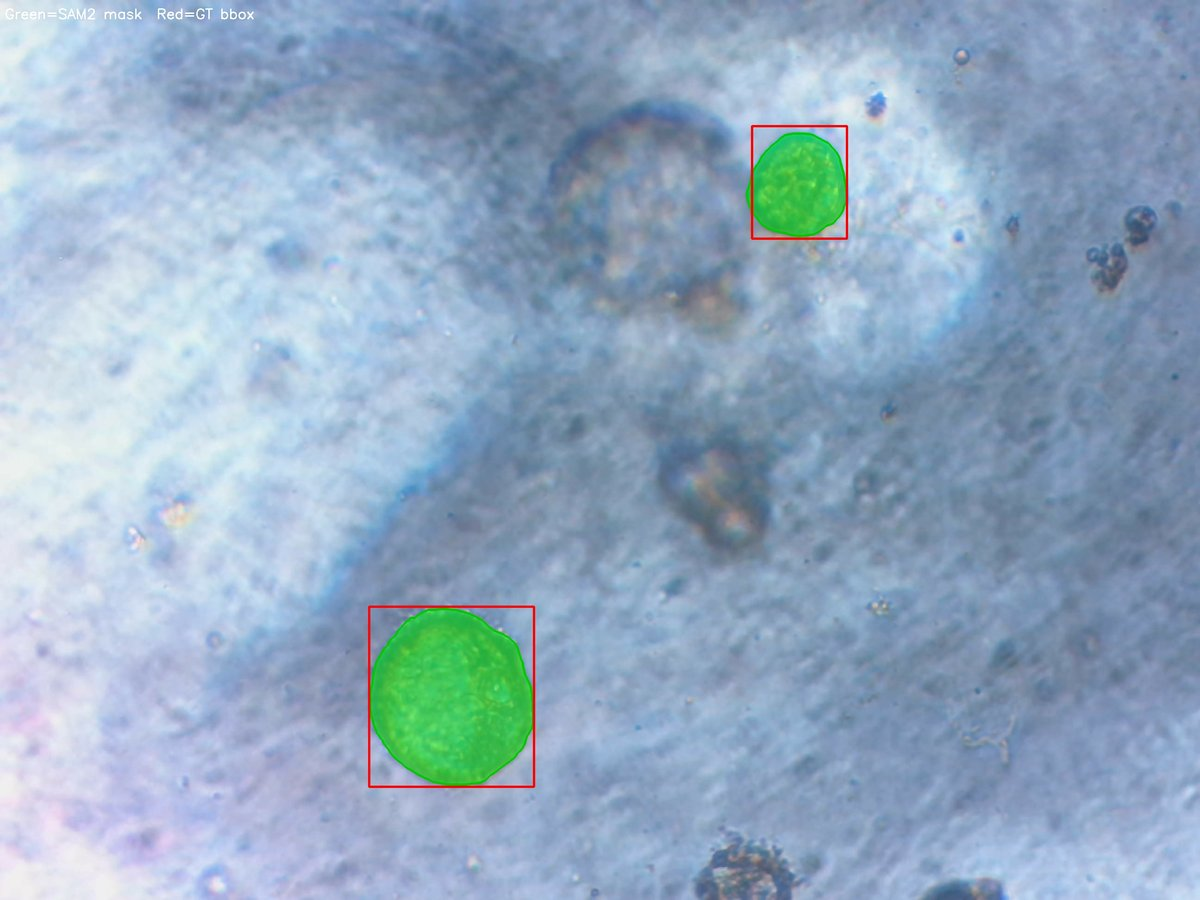
\includegraphics[width=\textwidth]{b1_full_seg.jpg}
      \vspace{-0.5em}
      \footnotesize B1 Full: F1=\textbf{1.00}
    \end{center}
    \column{0.32\textwidth}
    \begin{center}
      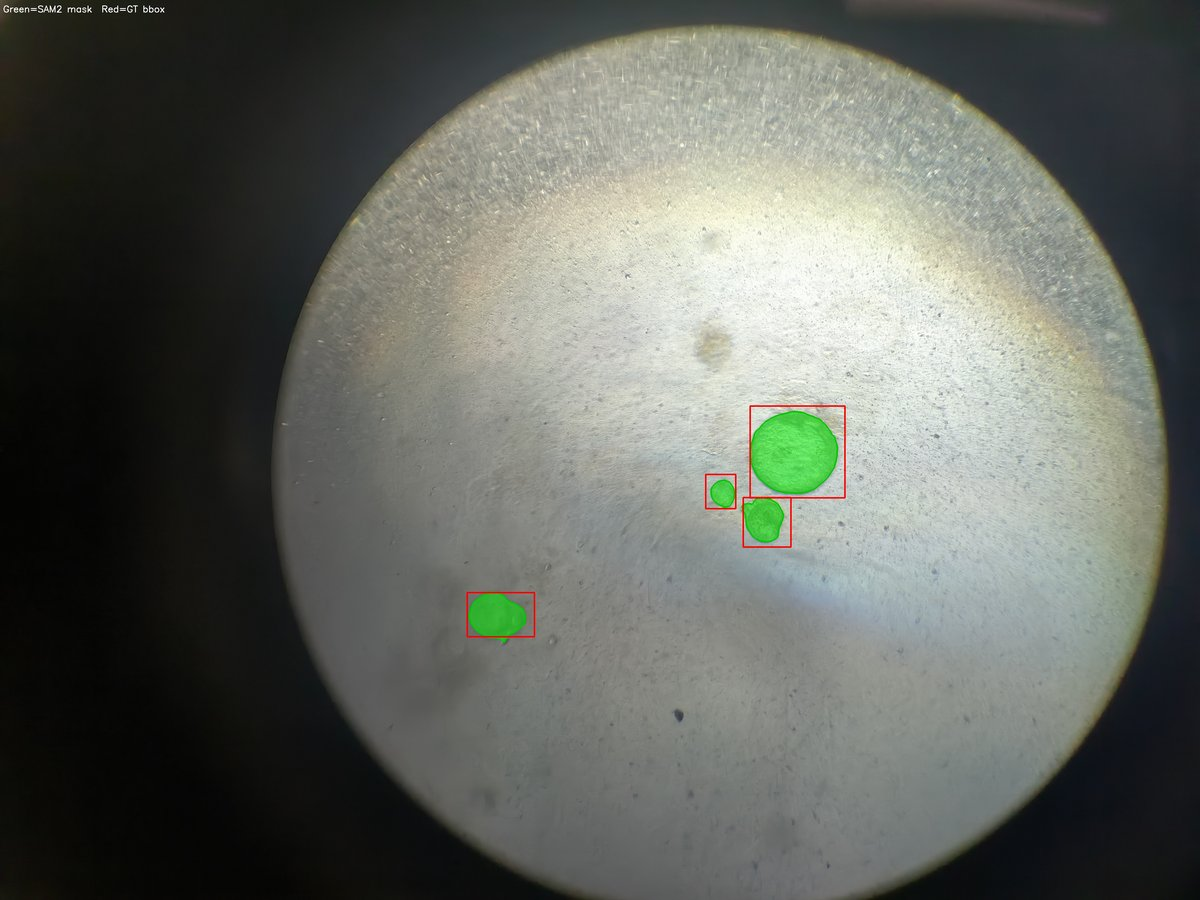
\includegraphics[width=\textwidth]{b2_full_seg.jpg}
      \vspace{-0.5em}
      \footnotesize B2 Full: F1=\textbf{0.80}
    \end{center}
    \column{0.32\textwidth}
    \begin{center}
      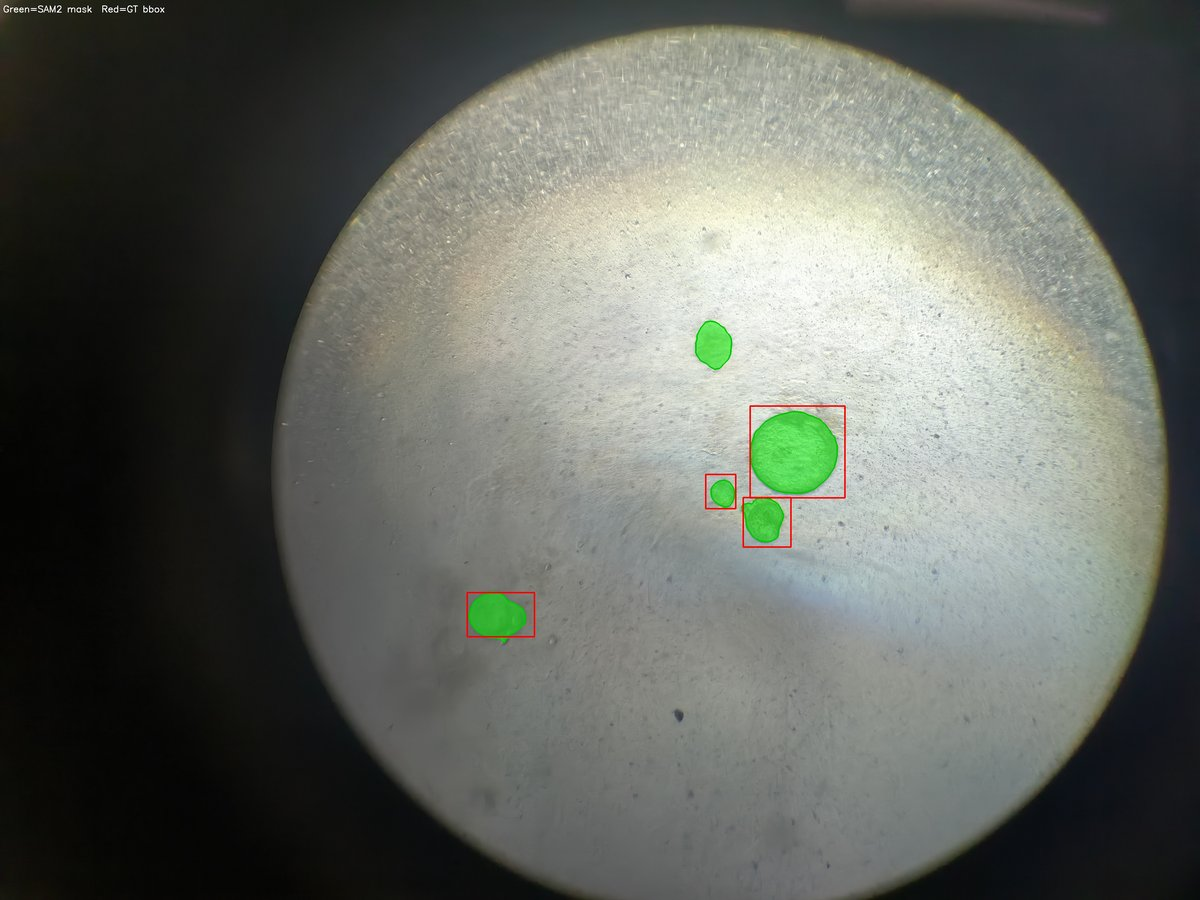
\includegraphics[width=\textwidth]{b2_fewshot_seg.jpg}
      \vspace{-0.5em}
      \footnotesize B2 Fewshot: F1=\textbf{0.92}
    \end{center}
  \end{columns}
  \vspace{0.3em}
  \begin{block}{可视化说明}
    \footnotesize 绿色填充 = SAM2 分割 mask；红色框 = GT bbox。B1（2592$\times$1944，大目标）完美检测。B2（4000$\times$3000，小目标）全量训练有 3 个 FP。B2 fewshot（B1 checkpoint + 3 张微调）仅 1 个 FP，\textbf{优于全量训练}。
  \end{block}
\end{frame}

\begin{frame}{鼠肝 v2：联邦学习四组策略}
  \begin{block}{FL 策略对比（YOLOv12n, 10 rounds $\times$ 10 local epochs）}
    \begin{tabular}{lllccccr}
      \toprule
      \textbf{Tag} & \textbf{Gate} & \textbf{Order} & \textbf{Final mAP50} & \textbf{Final mAP50-95} & \textbf{Best mAP50-95} & \textbf{Best@Rd} \\
      \midrule
      F1 & none & b1$\to$b2$\to$b3 & 0.30 & 0.24 & 0.26 & R3 \\
      F2 & soft (EWA) & b1$\to$b2$\to$b3 & 0.75 & 0.47 & 0.47 & R10 \\
      F3 & hard & b1$\to$b2$\to$b3 & \textbf{0.92} & \textbf{0.62} & 0.62 & R5 \\
      F4 & hard & b3$\to$b2$\to$b1 & 0.91 & 0.51 & 0.51 & R10 \\
      \bottomrule
    \end{tabular}
  \end{block}
  \vspace{0em}
  \begin{columns}[T]
    \column{0.48\textwidth}
    \begin{alertblock}{F3 hard gate 赢家}
      \begin{itemize}
        \item mAP50=0.92, mAP50-95=0.62
        \item R4 收敛后冻结（hard gate 阻断后续更新）
        \item b1 先跑建立强基座
      \end{itemize}
    \end{alertblock}
    \column{0.48\textwidth}
    \begin{block}{B2 修复前后 FL 对比}
      \begin{tabular}{lcc}
        \toprule
        & 修复前 & 修复后 \\
        \midrule
        F3 & 0.60 & \textbf{0.92} \\
        F4 & 0.10 & \textbf{0.91} \\
        F2 & 0.88 & 0.75 \\
        \bottomrule
      \end{tabular}
    \end{block}
  \end{columns}
\end{frame}

\begin{frame}{鼠肝 v2：FL 收敛曲线}
  \begin{block}{逐轮 mAP50 变化}
    \begin{tabular}{lcccccccccc}
      \toprule
      & R1 & R2 & R3 & R4 & R5 & R6 & R7 & R8 & R9 & R10 \\
      \midrule
      F1 (none) & .28 & .32 & .33 & .31 & .31 & .28 & .28 & .30 & .30 & .30 \\
      F2 (soft) & .28 & .32 & .35 & .35 & .35 & .58 & .65 & .67 & .72 & .75 \\
      F3 (hard) & .37 & .31 & .74 & \textbf{.92} & .92 & .92 & .92 & .92 & .92 & .92 \\
      F4 (hard) & .31 & .54 & .71 & .84 & .84 & .84 & .84 & .86 & .86 & .91 \\
      \bottomrule
    \end{tabular}
  \end{block}
  \vspace{0em}
  \begin{columns}[T]
    \column{0.48\textwidth}
    \begin{alertblock}{F3 hard gate: R4 跳跃}
      \begin{itemize}
        \item R3$\to$R4: 0.74$\to$0.92（+18pp 跳跃）
        \item R4 后完全冻结
        \item hard gate = 只接受优于当前的更新
      \end{itemize}
    \end{alertblock}
    \column{0.48\textwidth}
    \begin{block}{F2 soft gate: 平滑收敛}
      \begin{itemize}
        \item R5$\to$R6: 0.35$\to$0.58（开始加速）
        \item R10 仍在上升（未收敛）
        \item soft gate = EWA 加权聚合
      \end{itemize}
    \end{block}
  \end{columns}
\end{frame}

% ========================================================================
\section{MultiOrg 扩展实验}

\begin{frame}{Ensemble 实验：RF-DETR + YOLOv12}
  \begin{block}{三种融合策略结果}
    \begin{tabular}{lccc}
      \toprule
      策略 & mAP50 & mAP50-95 & vs RF-DETR \\
      \midrule
      RF-DETR 单模型 & 77.8\% & 48.8\% & — \\
      YOLOv12s 单模型 & 62.3\% & 37.2\% & $-$15.5pp \\
      \midrule
      WBF（SOTA 融合） & 63.2\% & 38.3\% & $-$14.5pp \\
      Intersection & 63.1\% & 39.7\% & $-$14.7pp \\
      Union & 70.0\% & 42.8\% & $-$7.8pp \\
      \bottomrule
    \end{tabular}
  \end{block}
  \begin{alertblock}{失败原因：YOLOv12s 是严格劣势模型}
    \begin{itemize}
      \item YOLO recall 80.4\% $\ll$ RF-DETR 96.2\%，无独有 TP
      \item Ensemble TP=4745 $<$ RF-DETR TP=4767 → YOLO 未补充任何 recall
      \item WBF 的 T/N 机制反而拉低 RF-DETR 高分 TP 的 score
      \item \textbf{结论：ensemble 需要两个精度接近的模型才能受益}
    \end{itemize}
  \end{alertblock}
\end{frame}

\begin{frame}{全面文献调研：MultiOrg SOTA}
  \begin{block}{MultiOrg 数据集 SOTA（mAP@0.5, t1\_b）}
    \begin{tabular}{llc}
      \toprule
      方法 & 来源 & mAP50 \\
      \midrule
      SSD & MultiOrg 论文 SOTA & 73.9\% \\
      YOLOv3 & MultiOrg 论文 & 70.3\% \\
      Faster R-CNN & MultiOrg 论文 & 68.4\% \\
      \textbf{RF-DETR（我们）} & \textbf{本研究} & \textbf{77.8\%} \\
      \bottomrule
    \end{tabular}
  \end{block}
  \begin{block}{其他 organoid 数据集 SOTA}
    \begin{tabular}{llcl}
      \toprule
      方法 & mAP50 & 数据集 & 数据量 \\
      \midrule
      Deliod & 87.5\% & Intestinal & — \\
      Orga-Dete & 81.4\% & Lung & 4008 张 \\
      Orga-Dete & 92.5\% & Duodenal & — \\
      Orga-Dete & 84.4\% & Murine intestinal & — \\
      OrgLine & N/A (PQ) & Multi-source & — \\
      \bottomrule
    \end{tabular}
  \end{block}
\end{frame}

\begin{frame}{Orga-Dete 三模块迁移实验：结果}
  \begin{alertblock}{结论：三模块全面失败，停止该方向}
    \begin{tabular}{lccc}
      \toprule
      \textbf{配置} & \textbf{mAP50} & \textbf{vs baseline} & \textbf{结论} \\
      \midrule
      yolo12s baseline & 62.3\% & — & 参考 \\
      yolo11n + MPCA & 44.2\% & — & 容量瓶颈 \\
      yolo11n + MPCA + EMASlideLoss & 44.0\% & $-$0.2pp & 噪声级 \\
      yolo12s + MPCA (random init) & 43.5\% & $-$18.8pp & 破坏预训练 \\
      yolo12s + MPCA (identity init) & 43.9\% & $-$18.4pp & init 不是根因 \\
      yolo12s + MPCA (identity) + EMASlideLoss & 44.5\% & $-$17.8pp & 噪声级 \\
      \bottomrule
    \end{tabular}
  \end{alertblock}
  \vspace{0em}
  \begin{block}{MPCA Identity Init 修复（commit 0cd3169）}
    \begin{itemize}
      \item \textbf{问题}：Sigmoid 随机初始化 $\approx$ 0.5 $\rightarrow$ 特征方差减半 $\rightarrow$ 破坏预训练
      \item \textbf{修复}：weight=0, bias=5 $\rightarrow$ sigmoid(5)$\approx$1.0 $\rightarrow$ output$\approx$x（identity）
      \item \textbf{验证}：std ratio 0.50$\rightarrow$0.99，预训练匹配 48.6\%$\rightarrow$99.2\%
      \item \textbf{但 mAP 几乎不变}（+0.38pp）——init 不是根因
    \end{itemize}
  \end{block}
\end{frame}

\begin{frame}{Orga-Dete 失败根因分析}
  \begin{columns}[T]
    \column{0.48\textwidth}
    \begin{block}{模型容量 vs mAP 强相关}
      \begin{tabular}{lc}
        \toprule
        模型 & mAP50 \\
        \midrule
        RF-DETR small (32M) & 77.8\% \\
        YOLOv12s (9.4M) & 62.3\% \\
        YOLOv11n+MPCA (2.6M) & 44.2\% \\
        YOLOv12s+MPCA (9.6M) & 43.9\% \\
        \bottomrule
      \end{tabular}
      \vspace{0.3em}
      
      每 3.5x 参数 $\approx$ +18pp
    \end{block}
    \column{0.48\textwidth}
    \begin{block}{五个根因}
      \begin{enumerate}
        \item \textbf{模型容量瓶颈}：2.6M vs 32M
        \item \textbf{MPCA 架构不兼容}：C3k2 vs A2C2f
        \item \textbf{单类检测无增益}：坐标注意力对多类有用
        \item \textbf{数据集差异}：4008张 vs 411张
        \item \textbf{BiFPN 未验证}：YAML 不兼容
      \end{enumerate}
    \end{block}
  \end{columns}
  \vspace{0em}
  \begin{alertblock}{铁律：乘性 Attention 必须 Identity Init}
    任何加在预训练模型上的乘性 attention 模块（SE、CBAM、CA、MPCA），初始状态必须是 identity，否则 sigmoid$\approx$0.5 会破坏预训练特征。验证方法：output/input std ratio $\approx$ 1.0。
  \end{alertblock}
\end{frame}

% ========================================================================
\section{联邦学习}

\begin{frame}{EWA 熵加权聚合策略}
  \begin{block}{核心思想}
    传统 FedAvg 按样本量均匀加权，忽略客户端模型质量差异。\\
    EWA 用验证集熵作为信号，\textbf{给更好的客户端更高权重}：
    \[
      w_c = \frac{\exp(-H_c / \alpha)}{\sum_{c'} \exp(-H_{c'} / \alpha)}
    \]
    其中 $H_c$ 是客户端 $c$ 在验证集上的预测熵，$\alpha$ 是温度参数。
  \end{block}
  \vspace{0em}
  \begin{block}{EWA Effective Interval 理论}
    \begin{itemize}
      \item \textbf{IID}：质量差异小 → EWA 退化 → \alert{无优势}
      \item \textbf{适度异质}：差异可区分 → EWA 最优 → \alert{+1.4\textasciitilde 1.5pp}
      \item \textbf{极端异质}：信号噪声大 → \alert{+1.1pp}
    \end{itemize}
  \end{block}
\end{frame}

% ========================================================================
\section{视觉原语方案}

\begin{frame}{视觉原语框架：范式转换}
  \begin{alertblock}{动机：bbox 范式到天花板}
    \begin{itemize}
      \item bbox 对不规则类器官只能参考定位，不能做分类判断
      \item SAHI / NMS / Soft-NMS 都是后处理治标
      \item \textbf{需要范式转换，不是渐进优化}
    \end{itemize}
  \end{alertblock}
  \vspace{0em}
  \begin{block}{视觉原语框架}
    \begin{tabular}{lll}
      \toprule
      \textbf{阶段} & \textbf{输入} & \textbf{输出} \\
      \midrule
      1. 检测 & 原图 & bbox (RF-DETR) \\
      2. 分割 & bbox + 原图 & 无类别 mask (SAM2 zero-shot) \\
      3. 形态学 & mask & primitive 向量 (面积/圆度/solidity) \\
      4. 语义确认 & mask + 原图 & VLM 推理 (是/否 organoid) \\
      5. FL 聚合 & primitive 分布 & 全局 primitive 分布 \\
      \bottomrule
    \end{tabular}
  \end{block}
  \vspace{0em}
  \begin{alertblock}{核心思想}
    FL 聚合的不是模型权重，而是\textbf{primitive 分布}。形态学特征不受像素尺度、成像设备影响。
  \end{alertblock}
\end{frame}

\begin{frame}{视觉原语方案：技术路线}
  \begin{columns}[T]
    \column{0.48\textwidth}
    \begin{block}{Step 1-2: 检测+分割（已完成）}
      \begin{itemize}
        \item RF-DETR: bbox 检测
        \item SAM2 zero-shot: mask 分割
        \item 鼠肝 B1: F1=1.00, mask F1=93.9\%
      \end{itemize}
    \end{block}
    \column{0.48\textwidth}
    \begin{block}{Step 3: 形态学特征}
      \begin{itemize}
        \item 面积/周长/圆度
        \item Solidity/Extent
        \item 长宽比/离心率
      \end{itemize}
    \end{block}
  \end{columns}
  \vspace{0em}
  \begin{columns}[T]
    \column{0.48\textwidth}
    \begin{block}{Step 4: VLM 语义确认}
      \begin{itemize}
        \item VLM 判断 mask 区域
        \item ``这是类器官吗?''
        \item 保留不确定性
      \end{itemize}
    \end{block}
    \column{0.48\textwidth}
    \begin{block}{Step 5: FL 聚合分布}
      \begin{itemize}
        \item 各 client primitive 直方图
        \item 全局 = 加权聚合
        \item 不共享权重，共享知识
      \end{itemize}
    \end{block}
  \end{columns}
  \vspace{0em}
  \begin{alertblock}{预期优势}
    不受像素尺度影响 $\to$ 跨域泛化；保留不确定性 $\to$ 避免强制决策；FL 聚合分布 $\to$ 隐私保护
  \end{alertblock}
\end{frame}


% ========================================================================
\section{CTM 持续思考实验}

\begin{frame}{CTM：连续思维机器（Sakana AI, NeurIPS 2025）}
  \begin{block}{核心创新}
    \begin{itemize}
      \item \textbf{NLMs}：每个神经元有私有权重（非共享）
      \item \textbf{神经同步化}：时间相关性矩阵（非快照），Q 从同步化来
      \item \textbf{Attention Q 从内部来}：模型自己决定看哪里（emergent active vision）
      \item \textbf{Loss}：argmin(loss) + argmax(certainty) $\to$ 自适应计算
    \end{itemize}
  \end{block}
  \vspace{0em}
  \begin{block}{架构}
    \begin{itemize}
      \item DINOv2 ViT-B/14 冻结（86.6M params, 0 trainable）
      \item CTM head 可训练（4.68M params）
      \item 输入 224$\times$224 $\to$ 257 spatial tokens $\to$ 20 ticks 推理
    \end{itemize}
  \end{block}
\end{frame}

\begin{frame}{CTM 全量训练结果（16198 crops, 50 epochs）}
  \begin{block}{Test set 2445 samples（按图像分割，0 泄露）}
    \begin{tabular}{lcc}
      \toprule
      \textbf{指标} & \textbf{AUC} & \textbf{说明} \\
      \midrule
      RF-DETR baseline & \textbf{0.893} & confidence 分数 \\
      CTM final tick & 0.800 & 第 20 tick \\
      CTM best tick & 0.801 & tick 17 \\
      CTM certain tick & 0.800 & argmax certainty per sample \\
      \bottomrule
    \end{tabular}
  \end{block}
  \vspace{0em}
  \begin{alertblock}{CTM 没超过 RF-DETR baseline（差 8.7pp）}
    \begin{itemize}
      \item Tick 1-2 AUC=0.20（反预测），tick 3 突跳 0.79
      \item 之后 15 tick 只涨 0.8pp — ``thinking'' 效果极弱
      \item Certainty 全程 $<$0.37，没有样本达到 0.8 阈值 — 自适应计算未启动
    \end{itemize}
  \end{alertblock}
\end{frame}

\begin{frame}{CTM 代码审计：5 个 Bug 修复}
  \begin{alertblock}{数据泄露（Critical）}
    按检测索引分割 train/val/test $\to$ 同图 crops 跨 split \\
    修复：按 \textbf{image\_name} 分割 $\to$ 0 泄露 \\
    效果：62 样本 val 0.907 $\to$ 2445 样本 test 0.800（水分 -10pp）
  \end{alertblock}
  \vspace{0em}
  \begin{alertblock}{同步化零值污染（Critical）}
    post\_acts\_history 预分配全零，每 tick 同步化混入当前 tick 的 0 值 \\
    $\to$ 破坏时间相关性矩阵 \\
    修复：改为 growing list，action synch 只看过去，output synch 看过去+当前
  \end{alertblock}
  \vspace{0em}
  \begin{block}{其他修复}
    \begin{itemize}
      \item acc\_best = acc\_certain 始终相同（都用 final tick）$\to$ 分别用 argmin/argmax
      \item auc\_certain = auc\_final（certain\_probs 算了没存）$\to$ 独立存储
      \item generate\_crops 重跑时 metadata 为空 $\to$ 已存在 crop 也加 metadata
    \end{itemize}
  \end{block}
\end{frame}


% ========================================================================
\section{视觉原语文献调研}

\begin{frame}{文献调研：关键论文发现}
  \begin{block}{核心论文}
    \begin{tabular}{llp{6cm}}
      \toprule
      \textbf{论文} & \textbf{会议} & \textbf{贡献} \\
      \midrule
      FORLA & NeurIPS 2025 & 联邦 slot attention，无监督跨域表征 \\
      TwVP & 2025 & 点/bbox 作为推理链中的空间原语 \\
      WIPES & ICCV 2025 & 小波频域视觉原语 \\
      Neuro-Symbolic & AAAI 2025 & 混合 CV + 逻辑推理消歧 \\
      CZSL Survey & 2025 & 属性$\times$物体原语组合泛化 \\
      \bottomrule
    \end{tabular}
  \end{block}
  \vspace{0em}
  \begin{alertblock}{核心洞察}
    \begin{itemize}
      \item 当前 TP/FP 在\textbf{全局特征空间}不可分（DINOv2 PR-AUC=0.29）
      \item 需要换一个特征空间：\textbf{object-centric 分解}（slot attention）
      \item FORLA 直接命中：FL + object-centric + slot attention
    \end{itemize}
  \end{alertblock}
\end{frame}

\begin{frame}{Phase 8-11 实验设计}
  \begin{block}{新增 4 个实验阶段}
    \begin{tabular}{llp{5cm}c}
      \toprule
      \textbf{Phase} & \textbf{方法} & \textbf{假设} & \textbf{成本} \\
      \midrule
      8 & 小波频域（WIPES） & TP/FP 频域可分 & 零（CPU 30min） \\
      9 & Slot Attention（FORLA） & object-centric 分解可分 & GPU 4-8h \\
      10 & 联邦原语聚合 & 分布聚合 $>$ 参数聚合 & 2-3 天代码 \\
      11 & 对比原语学习 & InfoNCE 强制拉开 TP/FP & 1 周 \\
      \bottomrule
    \end{tabular}
  \end{block}
  \vspace{0em}
  \begin{block}{决策树}
    Phase 8 PR-AUC $>$ 0.60 $\to$ 有效，进 Phase 9 提升 \\
    Phase 8 $<$ 0.50 $\to$ 无效，直接进 Phase 9 换特征空间 \\
    Phase 9 $>$ 0.50 $\to$ slot 有效，进 Phase 10 联邦 \\
    Phase 9 $<$ 0.50 $\to$ 进 Phase 11 对比学习
  \end{block}
\end{frame}


% ========================================================================
\section{Phase 8 小波实验结果}

\begin{frame}{Phase 8：小波频域原语分析（全量 16198 crops）}
  \begin{block}{实验结果}
    \begin{tabular}{llccc}
      \toprule
      \textbf{实验} & \textbf{特征空间} & \textbf{PR-AUC} & \textbf{ROC-AUC} & \textbf{维度} \\
      \midrule
      DINOv2 CLS（之前） & 768 维全局 embedding & 0.29 & — & 768 \\
      形态学（之前） & circ/solidity/ar & $<$0.50 & — & 4 \\
      \midrule
      W1: Haar 2L & 28 维小波统计 & \alert{0.457} & 0.681 & 28 \\
      W2: db4 3L & 40 维小波统计 & \alert{0.446} & 0.687 & 40 \\
      W3: haar+morph & 32 维拼接 & 0.645 & 0.791 & 32 \\
      \midrule
      \textbf{RF-DETR baseline} & confidence & \textbf{0.819} & \textbf{0.893} & 1 \\
      \bottomrule
    \end{tabular}
  \end{block}
  \vspace{0em}
  \begin{alertblock}{假设被推翻：小波单独无效}
    \begin{itemize}
      \item PR-AUC 0.45 $<$ 0.50（随机），100 crops 小样本 inflated 了结果
      \item 每个单特征 PR-AUC 都 $<$ 0.40（LL\_std=0.367 反预测）
      \item W3 morph 补救了（+18.8pp），说明形态学+小波有\textbf{互补性}
      \item 但仍远低于 RF-DETR 0.819
    \end{itemize}
  \end{alertblock}
\end{frame}


% ========================================================================
\section{Phase 9 Slot Attention 结果}

\begin{frame}{Phase 9：Slot Attention 原语提取（FORLA 路线）}
  \begin{block}{架构}
    \begin{itemize}
      \item DINOv2 ViT-B/14 冻结（86.6M params, 0 trainable）
      \item Slot Attention：K=8 slots, dim=128, 3 iters
      \item 可训练参数：480K（CTM 4.68M 的 1/10）
      \item 输入 224$\times$224 $\to$ DINOv2 spatial tokens [257,768] $\to$ Slot Attention $\to$ 8 slots [8,128] $\to$ classifier
    \end{itemize}
  \end{block}
  \vspace{0em}
  \begin{block}{训练（16198 crops, 50 epochs, 冬生 3060）}
    \begin{itemize}
      \item Train: 6316 (3158TP + 3158FP, balanced)
      \item Val: 2409 (666TP + 1743FP), Test: 2445 (805TP + 1640FP)
      \item 128s/epoch, early stop ep36 (patience=15)
      \item Best val AUC: 0.890 (ep21) $\approx$ RF-DETR 0.883
    \end{itemize}
  \end{block}
\end{frame}

\begin{frame}{Phase 9：Slot Attention 全方案对比}
  \begin{block}{Test set 结果（2445 samples）}
    \begin{tabular}{llccc}
      \toprule
      \textbf{方法} & \textbf{特征空间} & \textbf{ROC-AUC} & \textbf{PR-AUC} & \textbf{vs RF-DETR} \\
      \midrule
      \textbf{RF-DETR confidence} & 1 维 & \textbf{0.888} & \textbf{0.828} & baseline \\
      \textbf{Slot Attention} & 8$\times$128=1024 维 & \textbf{0.868} & \textbf{0.788} & \textbf{-2.0pp} \\
      CTM (20 ticks) & 4.68M & 0.800 & — & -8.8pp \\
      W3 haar+morph & 32 维 & 0.791 & 0.645 & -9.7pp \\
      Phase 5 k-NN (形态学) & 6 维 & 0.739 & — & -14.9pp \\
      W1 haar 2L & 28 维 & 0.681 & 0.457 & -20.7pp \\
      VLM (100 crops) & LLM 评分 & 0.713 & — & -17.5pp \\
      DINOv2 CLS & 768 维 & — & 0.29 & -53.8pp \\
      \bottomrule
    \end{tabular}
  \end{block}
  \vspace{0em}
  \begin{alertblock}{关键发现}
    \begin{itemize}
      \item Slot Attention 是\textbf{所有替代方案中最强的}（-2.0pp vs RF-DETR）
      \item Val AUC 0.890 $\approx$ RF-DETR 0.883 — val 上几乎追平
      \item 过拟合轻：train acc ep36=0.878（CTM ep2=1.0）
      \item 480K params，极轻量
    \end{itemize}
  \end{alertblock}
\end{frame}

\begin{frame}{Phase 9：决策树与下一步}
  \begin{block}{决策树结果}
    Phase 8 小波 PR-AUC = 0.45 $<$ 0.50 $\to$ 频域无效 \\
    Phase 9 Slot PR-AUC = \textbf{0.788 $>$ 0.50} $\to$ \textbf{object-centric 分解有效！}
  \end{block}
  \vspace{0em}
  \begin{alertblock}{缺失实验（高优先级）}
    \begin{itemize}
      \item \textbf{Slot + confidence 组合 AUC}：如果互补，combined 可能 $>$ 0.888
      \item \textbf{Phase 11 对比学习}：InfoNCE 强制拉开 TP/FP $\to$ 目标 PR-AUC $>$ 0.85
      \item \textbf{Phase 10 联邦 slot 聚合}：FORLA + FedCtx HNSW
    \end{itemize}
  \end{alertblock}
  \vspace{0em}
  \begin{block}{为什么 Slot Attention 有效？}
    \begin{itemize}
      \item DINOv2 CLS = 全局 embedding，TP/FP 完全重叠（PR-AUC=0.29）
      \item Slot Attention = object-centric 分解，每个 slot 学一个物体组件
      \item TP 有 organoid 内部纹理结构 $\to$ slot 捕获
      \item FP 是背景碎片 $\to$ slot 不同
    \end{itemize}
  \end{block}
\end{frame}


% ========================================================================
\section{Phase 11 SupCon + C4 闭环}

\begin{frame}{Phase 11：SupCon 对比学习（$\beta$ 消融）}
  \begin{block}{Loss = CE + $\beta \times$ SupCon}
    \begin{itemize}
      \item SupCon (Khosla NeurIPS 2020)：TP-TP embedding 拉近，TP-FP 推远
      \item Projection head: 128 $\to$ 256 $\to$ L2 normalize
      \item $\beta=0.5$：SupCon 贡献 1.6 = CE 的 3x $\to$ 压制分类头
      \item $\beta=0.1$：SupCon 贡献 0.32 $\to$ CE 主导，SupCon 辅助
    \end{itemize}
  \end{block}
  \vspace{0em}
  \begin{alertblock}{$\beta$ 消融结果（$\tau=0.07$ 固定）}
    \begin{tabular}{lccc}
      \toprule
      \textbf{指标} & \textbf{Phase 9} & \textbf{$\beta=0.5$} & \textbf{$\beta=0.1$} \\
      \midrule
      Slot AUC & 0.868 & 0.845 & \textbf{0.860} \\
      Embedding AUC & --- & 0.859 & \textbf{0.868} \\
      Combined AUC & 0.903 & 0.909 & \textbf{0.910} \\
      Combined PR-AUC & 0.853 & 0.860 & \textbf{0.862} \\
      Val best AUC & 0.890 & 0.917 & \textbf{0.922} \\
      \bottomrule
    \end{tabular}
  \end{alertblock}
\end{frame}

\begin{frame}{C4 闭环验证：Slot 过滤提升检测 AP}
  \begin{block}{实验设计（方案 \S 7.6）}
    \begin{itemize}
      \item 用 SupCon 训练的 slot encoder 对 RF-DETR 检测框打分
      \item 4 种过滤策略搜索最优参数
      \item 评估指标：PR-AUC（=AP50 近似）
    \end{itemize}
  \end{block}
  \vspace{0em}
  \begin{alertblock}{结果（$\beta=0.1$ embeddings）}
    \begin{tabular}{lccc}
      \toprule
      \textbf{策略} & \textbf{AP} & \textbf{$\Delta$ AP} & \textbf{参数} \\
      \midrule
      Baseline (RF-DETR conf) & 0.829 & --- & --- \\
      Hard filter & 0.834 & +0.5pp & thr=0.10 \\
      Soft penalize ($\alpha$=0.5) & 0.860 & +3.1pp & conf$\times(1-0.5(1-s))$ \\
      \textbf{Geometric mean} & \textbf{0.861} & \textbf{+3.3pp} & $conf^{0.8} \times slot^{0.2}$ \\
      LR meta (5-fold) & 0.857 & +2.9pp & 5-fold LR \\
      \bottomrule
    \end{tabular}
  \end{alertblock}
  \vspace{0em}
  \begin{block}{结论}
    RF-DETR AP 0.829 $\to$ 0.861（\textbf{+3.3pp}）\\
    最优权重 $w_{slot}=0.20$（和 Phase 9 组合分析一致）\\
    \textbf{C4 验证成功}：slot encoder 提升检测 mAP
  \end{block}
\end{frame}

\begin{frame}{Phase 10：联邦 Slot 聚合（真 Plate$\times$Class）}
  \begin{block}{6 个真实 client}
    \begin{tabular}{lcccccc}
      \toprule
      \textbf{Client} & \textbf{N} & \textbf{TP\%} & \textbf{Local} & \textbf{Global} & \textbf{$\Delta$} & \textbf{Conf} \\
      \midrule
      Macros\_P23 & 328 & 23\% & 0.697 & \textbf{0.754} & \textbf{+5.7pp} & 0.891 \\
      Normal\_P31 & 207 & 28\% & 0.792 & \textbf{0.830} & \textbf{+3.8pp} & 0.900 \\
      Normal\_P37 & 283 & 17\% & 0.836 & 0.830 & -0.6pp & 0.915 \\
      Macros\_P4 & 772 & 40\% & 0.821 & 0.810 & -1.1pp & 0.874 \\
      Normal\_P15 & 597 & 39\% & 0.890 & 0.887 & -0.3pp & 0.919 \\
      Normal\_P4 & 258 & 33\% & 0.896 & 0.885 & -1.0pp & 0.903 \\
      \midrule
      Mean & --- & --- & 0.822 & \textbf{0.833} & \textbf{+1.1pp} & 0.900 \\
      \bottomrule
    \end{tabular}
  \end{block}
  \vspace{0em}
  \begin{alertblock}{关键洞察}
    \begin{itemize}
      \item 小 client / 低 TP 率获益最大（Plate\_23 +5.7pp）
      \item 大 client 不获益（本地数据已足够）
      \item Combined (kNN+conf) ROC=0.907（+1.9pp vs RF-DETR）
      \item ``数据不动，知识动''：只共享 256 维 embedding
    \end{itemize}
  \end{alertblock}
\end{frame}

\begin{frame}{跨域泛化：MultiOrg $\to$ 鼠肝 \& Intestinal（结果）}
  \begin{block}{实验设置}
    \begin{itemize}
      \item SupCon checkpoint: MultiOrg 100 crops 训练（K=8, dim=128, $\tau$=0.07, $\beta$=0.1）
      \item 评估: DINOv2 ViT-B/14 提取 embedding $\to$ slot attention $\to$ AUC/AP
      \item 鼠肝: RF-DETR Small 检测（3 batch checkpoint），Intestinal: YOLOv12s 检测
    \end{itemize}
  \end{block}
  \vspace{0em}
  \begin{alertblock}{DINOv2 跨域结果：Slot 失效 + LOO 真跨域}
    \footnotesize
    \begin{tabular}{lccccc}
      \toprule
      \textbf{数据集} & \textbf{单域} & \textbf{同域} & \textbf{LOO} & \textbf{Conf} & \textbf{泄露} \\
      \midrule
      鼠肝 B1 & \textcolor{red}{0.29} & 0.74 & \textcolor{red}{0.49} & 0.91 & 0.25 \\
      鼠肝 B2 & \textcolor{red}{0.51} & 0.70 & \textcolor{red}{0.56} & 0.98 & 0.14 \\
      鼠肝 B3 & \textcolor{red}{0.54} & 0.85 & 0.82 & 0.92 & 0.03 \\
      Intestinal & 0.67 & 0.74 & \textcolor{red}{0.58} & 0.92 & 0.16 \\
      \bottomrule
    \end{tabular}
  \end{alertblock}
  \vspace{0em}
  \begin{block}{诊断}
    \begin{itemize}
      \item 同域结果有数据泄露（平均虚高 0.14pp）
      \item LOO 真跨域：B1/B2 接近随机，Intestinal 比单域还差
      \item \textbf{根因}：DINOv2 全局特征是域特定的，不构成通用 organoid 原语
    \end{itemize}
  \end{block}
\end{frame}

\begin{frame}{CLIP 语义对齐：Zero-Shot 跨域有信号}
  \begin{block}{动机：借鉴 NLP 语义分析成功经验}
    \begin{itemize}
      \item NLP 跨域成功 = 大规模预训练 + 语义对齐 + CoT 推理
      \item DINOv2 有预训练但\textbf{无语义对齐}——纯视觉特征域特定
      \item CLIP 有文本-视觉对齐空间 → ``a real organoid'' vs ``background''
    \end{itemize}
  \end{block}
  \vspace{0em}
  \begin{alertblock}{CLIP Zero-Shot 结果（无训练！）}
    \footnotesize
    \begin{tabular}{lcccc}
      \toprule
      \textbf{数据集} & \textbf{DINOv2 单域} & \textbf{DINOv2 LOO} & \textbf{CLIP zero-shot} & \textbf{Conf} \\
      \midrule
      MultiOrg & 0.79 & — & 0.73 & 0.87 \\
      鼠肝 B1 & \textcolor{red}{0.29} & 0.49 & \textbf{0.86} & 0.91 \\
      鼠肝 B2 & 0.51 & 0.56 & \textbf{0.66} & 0.98 \\
      鼠肝 B3 & 0.54 & 0.82 & \textbf{0.69} & 0.92 \\
      \bottomrule
    \end{tabular}
  \end{alertblock}
  \vspace{0em}
  \begin{block}{关键发现}
    \begin{itemize}
      \item B1 从 0.29 $\to$ \textbf{0.86}（+0.57），zero-shot 差 conf 仅 5.8pp
      \item CLIP \textbf{无需训练}，仅用文本 prompt 就能跨域区分 TP/FP
      \item ``morphological'' prompt 在鼠肝最优，``medical'' 在 MultiOrg 最优
    \end{itemize}
  \end{block}
\end{frame}

\begin{frame}{训练破坏泛化：SupCon / CoOp LOO 结果}
  \begin{alertblock}{所有监督训练都破坏 CLIP zero-shot 跨域能力}
    \scriptsize
    \begin{tabular}{lccccc}
      \toprule
      \textbf{数据集} & \textbf{DINOv2 LOO} & \textbf{CLIP zero-shot} & \textbf{CLIP+SupCon} & \textbf{CoOp} & \textbf{Conf} \\
      \midrule
      MultiOrg & — & 0.73 & 0.95 & 0.62 & 0.87 \\
      鼠肝 B1 & 0.49 & \textbf{0.86} & 0.50 & 0.67 & 0.91 \\
      鼠肝 B2 & 0.56 & \textbf{0.66} & 0.57 & 0.58 & 0.98 \\
      鼠肝 B3 & 0.82 & \textbf{0.69} & 0.45 & 0.65 & 0.92 \\
      Intestinal & 0.58 & \textbf{0.69} & 0.50 & 0.69 & 0.92 \\
      \midrule
      \textbf{平均} & 0.58 & \textbf{0.73} & 0.58 & 0.64 & \textbf{0.94} \\
      \bottomrule
    \end{tabular}
  \end{alertblock}
  \vspace{0em}
  \begin{block}{核心结论}
    \begin{itemize}
      \item CLIP zero-shot（无训练）= 最强跨域 slot（平均 0.73）
      \item SupCon 训练 slot $\to$ B1 从 0.86 $\to$ 0.50（\textcolor{red}{-0.36}）
      \item CoOp 训练 prompt $\to$ B1 从 0.86 $\to$ 0.67（\textcolor{red}{-0.19}，破坏更少但仍不如 zero-shot）
      \item 和 NLP 一致：微调破坏预训练 zero-shot 泛化
      \item $\to$ \textbf{不训练参数}，改用 prompt 工程 / VLM 推理 / 3D 时序
    \end{itemize}
  \end{block}
\end{frame}


% ========================================================================
\section{总结}

\begin{frame}{总结}
  \begin{columns}[T]
    \column{0.48\textwidth}
    \begin{block}{已完成}
      \begin{itemize}
        \item[\checkmark] SOTA 全面调研 + MultiOrg 77.8\%
        \item[\checkmark] SAM2 三轮 + FP 抑制 + Ensemble 均失败
        \item[\checkmark] 鼠肝 v2 14 实验 + bbox FL 完成
        \item[\checkmark] CTM 全量训练：AUC=0.80（$<$RF-DETR）
        \item[\checkmark] Phase 8 小波：假设被推翻
        \item[\checkmark] \textbf{Phase 9 Slot：PR-AUC=0.788}
        \item[\checkmark] \textbf{Phase 9 组合：AP 0.903}（+1.5pp）
        \item[\checkmark] \textbf{Phase 11 SupCon $\beta=0.1$：AP 0.910}
        \item[\checkmark] \textbf{C4 闭环：AP 0.829$\to$0.861}（+3.3pp）
        \item[\checkmark] \textbf{Phase 10 联邦：Global$>$Local +1.1pp}
        \item[\checkmark] 视觉原语文献调研（FORLA/TwVP/WIPES）
        \item[\checkmark] \textbf{跨域评估：4场景全部失效}
        \item[\checkmark] \textbf{LOO 真跨域：DINOv2 仍然失败}
        \item[\checkmark] \textbf{CLIP zero-shot：B1 0.29$\to$0.86（+0.57）}
        \item[\checkmark] \textbf{训练破坏泛化：SupCon/CoOp 都不如 zero-shot}
      \end{itemize}
    \end{block}
    \column{0.48\textwidth}
    \begin{alertblock}{核心成果}
      \begin{itemize}
        \item RF-DETR AP: 0.829 $\to$ \textbf{0.861}（+3.3pp）
        \item Combined ROC: \textbf{0.910}（+2.2pp）
        \item 联邦聚合：小 client +5.7pp
        \item \textcolor{red}{DINOv2 跨域失效}，\textbf{CLIP 语义对齐有效}
        \item \textbf{所有训练都破坏 zero-shot 泛化}
        \item CLIP zero-shot 平均 0.73 = 最强跨域
      \end{itemize}
    \end{alertblock}
  \end{columns}
  \vspace{0em}
  \begin{alertblock}{下一步}
    \begin{itemize}
      \item B2: VLM 两步推理（TwVP 范式，API 待恢复）
      \item Prompt 工程 / 多 prompt 集成（无训练优化）
      \item C1: 3D 时序数据集（OrganoID 4-day tracking）
      \item 论文撰写 + 专利申请
    \end{itemize}
  \end{alertblock}
\end{frame}


\begin{frame}{未来工作：数据集扩展计划}
  \begin{block}{已使用数据集}
    \begin{tabular}{lccc}
      \toprule
      \textbf{数据集} & \textbf{张数} & \textbf{类型} & \textbf{状态} \\
      \midrule
      Intestinal (Deliod) & — & 肠道类器官 & \checkmark 超 SOTA 88.1\% \\
      鼠肝 B1/B2/B3 & 40 & 鼠肝类器官 & \checkmark 完成 \\
      MultiOrg & 411 & 多类器官 & \checkmark 超 SOTA 77.8\% \\
      \bottomrule
    \end{tabular}
  \end{block}
  \vspace{0em}
  \begin{block}{计划扩展数据集}
    \begin{tabular}{lcc}
      \toprule
      \textbf{数据集} & \textbf{特点} & \textbf{目标} \\
      \midrule
      肠/肺/脑类器官 & 不同器官类型 & 跨器官泛化 \\
      多实验室鼠肝 & 不同显微镜/染色 & 预处理标准化 \\
      多倍率 (4X/10X/20X) & 分辨率差异 & 尺度不变性 \\
      共聚焦/荧光 & 不同成像方式 & 跨模态 FL \\
      \bottomrule
    \end{tabular}
  \end{block}
  \vspace{0em}
  \begin{alertblock}{核心方向}
    预处理标准化 $\to$ 视觉原语 $\to$ FL 聚合 $\to$ 数据飞轮
  \end{alertblock}
\end{frame}

\begin{frame}[allowframebreaks]{参考文献}
  \footnotesize
  \begin{thebibliography}{99}
    \bibitem{bukas2024} Bukas et al. \textit{MultiOrg: A Multi-rater Organoid-detection Dataset}. NeurIPS, 2024.
    \bibitem{tian2025} Tian et al. \textit{YOLOv12: Attention-Centric Real-Time Object Detectors}. arXiv:2502.12524, 2025.
    \bibitem{solawetz2025} Solawetz et al. \textit{RF-DETR: Real-Time DEtection TRansformer}. ICLR, 2026.
    \bibitem{bodla2017} Bodla et al. \textit{Soft-NMS -- Improving Object Detection with One Line of Code}. ICCV, 2017.
    \bibitem{akyon2022} Akyon et al. \textit{Slicing Aided Hyper Inference (SAHI)}. CVPRW, 2022.
    \bibitem{bulten2021} Bulten et al. \textit{Overcoming the Limitations of Patch-based Learning to Detect Cancer in Whole Slide Images}. PMC, 2021.
    \bibitem{lu2025} Lu et al. \textit{Thinking with Visual Primitives}. DeepSeek-AI, 2025.
    \bibitem{kirillov2023} Kirillov et al. \textit{Segment Anything (SAM)}. ICCV, 2023.
    \bibitem{solovyev2021} Solovyev et al. \textit{Weighted Boxes Fusion: Ensembling boxes from different object detection models}. IVC, 2021.
    \bibitem{huang2025} Huang et al. \textit{Orga-Dete: An Improved Lightweight Deep Learning Model for Lung Organoid Detection}. Applied Sciences, 2025.
    \bibitem{deng2026} Deng et al. \textit{OrgLine: A versatile pipeline for organoid morphometry using detector-guided prompts}. Cell Reports Methods, 2026.
  \end{thebibliography}
\end{frame}

\begin{frame}[plain]
  \centering
  \vfill
  \Large\textcolor{myblue}{Thank You!}\\[0.8em]
  \normalsize Questions \& Discussion\\[1.5em]
  \footnotesize\texttt{github.com/dechang64/organoid-fl}
  \vfill
\end{frame}
\end{document}
